\documentclass{article}
\usepackage[dvips]{graphicx}
\author{David J. Burger}
\title{Loose Dog Operational Transformations}
\begin{document}
\maketitle

\section{Introduction}

Computer applications which facilitate collaboration between
individuals are nothing new.  Email and internet relay chat are two
such applications that have been around for many years.  More
recently, however, distributed applications are being built that allow
for a far greater degree of collaboration.  These applications allow
persons at distributed locations to simultaneously edit a live
document via a communications network.  This paper will describe
the system developed to provide this functionality in the Loose
Dog system.  Loose Dog is the name for the communications and
synchronization system in the House Party collaborative application
framework.  The first section will look at various
synchronization strategies currently in use, giving their advantages
and disadvantages.  The second section will explain operational
transformations, the technique I have employed in the Loose Dog system.
A brief history of operational transformations will also be given.
Following that will be a section on specific Loose Dog operational
transformation implementation details.  The final section provides a
conclusion and addresses possible future modifications to the system.

\section{Synchronization Strategies}

Strategies for providing live document editing in a distributed
environment fall into four major categories: single active
participant, locking, transactions, and operational transformations.
Each strategy is subject to various trade offs.

The single active participant strategy is a strategy that is
reminiscent of the now disappearing token ring networking technology.
With token ring networking, a single computer held the ``token'' and
was free to communicate on the shared communications medium.  All
other computers were expected to remain silent.  After a brief period
of time the token would be passed on to the next computer.  Similarly,
the single active participant strategy allows only one computer at a
time to have modification access to the shared document.  The means by
which access to the document is controlled may be through software or
through an externally defined protocol.  This strategy has a major
drawback in that free editing of the document is prevented as
participants wait to become the active participant.  Conflicting
operations are possible with this strategy if an externally defined
access protocol is being used and participants fail to follow the
protocol.  When the policy is followed correctly, or when a software
controlled access mechanism is used, conflicts can be avoided
completing, thus making this strategy easier to implement.

Locking is a strategy that, not surprisingly, requires data to be locked
before it can be modified.  Locking is a technique that is widely used
in the world of databases.  When data is locked any other
participant's requests to acquire a lock on the same data will be
prevented, therefore eliminating the possibility of conflicting
modifications.  The acquisition of locks requires a round trip to
determine the success or failure of acquiring the lock.  When the lock
is denied, a situation similar to the single active participant occurs
and the user will be forced to wait to make modifications to the data
in question.  Even when the lock is granted, the hesitation in
acquiring the lock results in a degradation of the user's experience.
The locking strategy also requires developers to make difficult
choices on the granularity of the locks they will use.  Fine
granularity locks, for example requiring a lock for each character of
a text document, requires a high number of round trip lock acquisition
requests.  This becomes a limiting factor and requires a highly responsive
network.  Larger granularity locks increase the possibility of
participants being denied the lock and therefore having to wait for
the lock to be released.  In the worst case the
interactivity of the document begins to approach that of the single
active participant strategy.

Transactions, like locking, is a technique commonly used in database
technology.  Transactions allow the user to make modifications to a
local copy of the shared document immediately with those changes being
sent to a central server.  If conflicting operations are detected at
the server the transaction is denied, and the client is forced to roll
back the local document to the pre-transaction state.  Transactions
can be implemented using locks or time stamps to prevent or recognize
conflicting operations.  When locks are used, the problems noted above
about locking also apply to transactions.  Regardless of how they are
implemented, transactions suffer from the major problem that a user's
actions may need to be rolled back.  A transaction roll back, while
natural in a database system, is disconcerting to the editors of a
shared document.  Transactions seem to be inappropriate for
interactive use.

The most modern strategy, and the one that I have deployed in the
Loose Dog system, is called operational transformations.
Operational transformations provide each client immediate access to the
shared document, with local edits being applied immediately.  The
edits, or operations, are then sent to all the other participants.
Because the operations are applied locally and then sent to other
clients immediately it is quite likely that conflicting operations will
occur.  When this happens, the operations must be transformed in such
a way that the participant's documents converge to a common state,
thus the name ``operational transformation.''  This strategy has the
benefit of providing a real time document editing experience for the
users, however, it can be substantially more complicated to
implement than the strategies described above.  The next section
will provide a brief history of operational transformations along with
more details on how operational transformations work.

\section{Operational Transformations}

The pioneering application in the field of operational transformations
was the GROVE system by C. A. Ellis and S. J. Gibbs developed at the
Microelectronics and Computer Technology Corporation (MCC) in Austin,
Texas \cite{grove}.  GROVE, which stands for GRoup Outline Viewing
Editor, allowed distributed participants to simultaneously edit a
shared outline.  GROVE allowed real time editing of the outline with
conflicting operations transformed to allow for convergence of the
outline.  An example of a conflicting operation that could occur on an
outline is when one participant deletes the second word of an outline
item while another user adds a word after the tenth word in the same
outline item.  For convergence of the document the position of the
word insert will need to be adjusted to the left by the number of
characters deleted in the second word.  The algorithm that Ellis and
Gibbs created was known as the Distributed Operational Transform
(dOPT).

Several research groups carried on independent exploration of
operational transformations throughout the nineties.
Out of this work came a variety of modifications and
improvements to Ellis' and Gibbs' operational transformation
algorithms.  The most notable of these include the REDUCE (REal-time
Distributed Unconstrained Cooperative Editing) system \cite{reduce},
the Jupiter system \cite{jupiter}, and the adOPTed algorithm
\cite{adopted}.

While Ellis' and Gibbs' dOPT has evolved into a variety of algorithms,
the basic idea remains the same.  A partial ordering is made of the
operations that occur in the system.  For operations in which a
precedence can be determined, the proper execution ordering is
applied.  For those operations in which a precedence cannot be
determined, operational transformations are used to produce operations
that lead to document convergence.

To determine a partial ordering, each locally generated operation
includes auxiliary information when sent to the other participants.
This information typically takes the form of a state vector.  The
state vector has a numeric entry for each participant that indicates
how many operations have been received from that participant's site.
When an operation is received from the network, the included state
vector can be examined to determine if the client that generated the
operation has executed operations that have not been executed by the
receiving site.  If this is the case, the operation is deemed a
``future operation'' and is queued until the missing operations arrive
allowing for its execution.  If the state vector included in the
received operation matches the local state vector the operation is
ready for immediate execution.  If the received state vector indicates
that the receiving site has executed operations not executed by the
sending site of an operation the operation is deemed a ``past
operation'' and the operation may have to be transformed before being
applied locally.  A diagram of this process can be seen in
Figure~\ref{flow}.

\begin{figure}[!h]
\begin{center}
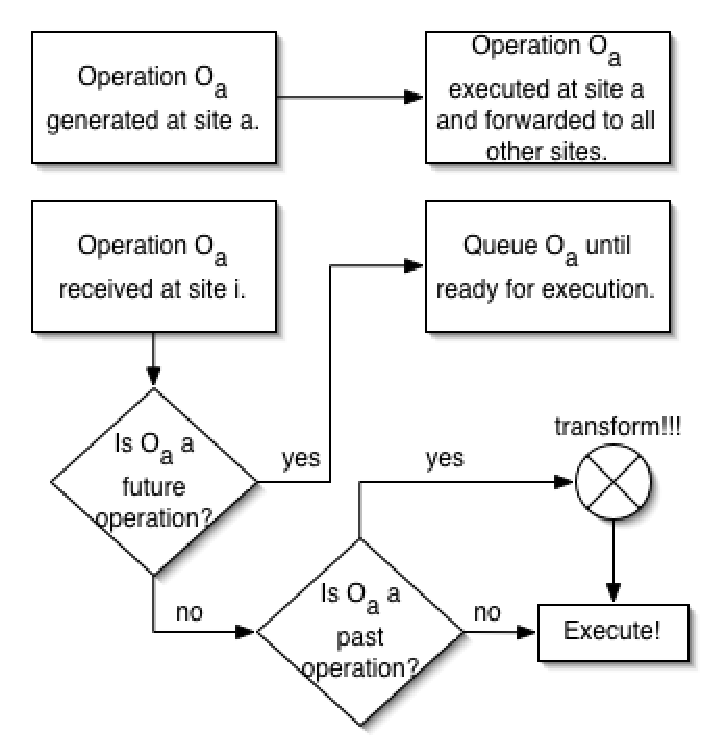
\includegraphics{flow.eps}
\caption{General Operational Transformation Process} \label{flow}
\end{center}
\end{figure}

There are three primary data structures used in the implementation of
an operational transformation system.  As described above, a state
vector must be kept to track the number of operations that have been
generated at each site.  This state vector is included in each
operation request sent over the network so that a partial ordering of
the operations can be determined.  Delaying future operations until
missing operations have arrived is achieved by holding a queue of
such operations.  When operations arrive and are executed this queue
will be examined to see if any of the queued future operations are now
ready for execution.  Lastly, a log, or history buffer, must be kept
of executed operations.  The history buffer is kept so that past
operations can be transformed against it.  The arriving past
operations will need to be transformed against any operations in the
history buffer that were not accounted for by the site generating the
past operation.

Currently programs that use operational transformation techniques seem
to be leaving the realm of research projects and entering the realm of
everyday applications.  Users of the OS X operating system may be
interested in trying out SubEthatEdit \cite{subetha}, formerly known
as Hydra.  SubEthaEdit is a group editor designed for pair programming
and is free for non-commercial use.  Members of Xerox PARC Jupiter
team spun off a startup called PlaceWare.  Recently PlaceWare was
purchased by Microsoft and the result appears to be a product called
Live Meeting \cite{livemeeting}.

\section{Implementation}

The first decision to be made when applying operational transformation
technology to the House Party framework via the Loose Dog system was
which general algorithm to follow.  Several algorithms had been
proposed as extensions to, and improvements of, the original dOPT
algorithm by Ellis and Gibbs.  These algorithms can be separated into
two different networking topologies: fully distributed and star
topologies.

The usage of a fully distributed algorithm adds several complexities.
One such complexity is the issue of how participants join a session.
Unlike a star topology, in which a client connects to a single
centralized computer, in a fully distributed system a more complex
join operation must occur.  During this operation, the client must
discover the addresses of all the other participating clients and make
connections to them.  Getting the initial state of the document can
also be a problem as operations currently in transit in the system can
have each client's individual document in a different state.  A fully
distributed system also has the problem of the ever growing history
buffer.  In order to remove outdated entries in the history buffer the
system must be known to be in a state with no operations in transit,
that is in a state of quiescence.  Algorithms exist to determine
quiescence, however, site failures and a variable number of
participants complicate this process greatly.

With a star topology participant sites only communicate directly with
a centralized server.  This eliminates several of the complexity
inducing problems of a fully distributed system.  The join process is
greatly simplified as a client participant must make only one
connection.  The initial state of the shared document is also easily
available to joining participants directly from the centralized server.
Because the star topology allows each participant to act as if it is
synchronizing with only one other client, that is the centralized
server, much of the complexity in being prepared to handle an
operation from any client at any time is removed.  An example of this
is the elimination of the growing history buffer problem.  With a star
topology we must only store a participants outgoing operations in
preparation for transformation.  The size of the outgoing queue is
easily managed as an operation in the queue can be discarded as soon
as an operation arrives from the server acknowledging that operation.
The one major drawback to the star topology is that it has a central
point of failure.

The current design of the messaging library in the Loose Dog system
does not contain built in mechanisms for managing a distributed
network of client computers.  Because of this, and the inherent
advantages stated above, it became clear that the only logical choice
for the operational transformation in the Loose Dog system would be to
use a star topology.

The authoritative implementation of operational transformations in a
star topology network is the Jupiter collaborative system designed by
Nichols, Curtis, Dixon, and Lamping at Xerox PARC.  The Jupiter system
is a ``multi-user, multimedia, virtual world intended to support
long-term remote collaboration.''  Many of the implementation details
of the operational transformations in the Loose Dog system were
derived from the ideas in the Jupiter system.

The first thing that was done to create operational transformations
for the Loose Dog system was to create an \textbf{OpTrans} class that
holds the necessary data structures.  This includes the
\textbf{myMsgs} and \textbf{otherMsgs} integer fields.  These fields
perform the function of the state vectors in the general operational
transformation algorithm.  A value is not necessary for each connected
client because with the star topology, any received message can be
treated as if it were generated by the server.  The other primary data
structure in the \textbf{OpTrans} class is the outgoing linked list.
This is the list that is used to hold operations that have been
generated locally.  These operations may be needed later to perform
operational transformations on arriving operations.

It was then decided that the best way to integrate operational
transformations into the Loose Dog system was to have the operational
transformations act as a filter.  On reception, a message would be
directed through the filter's receive method.  Likewise, on sending, a
message would be directed through the filter's send method.  The
benefit of this filter like approach is that it would be possible to
integrate into the existing House Party framework with little
disruption to the existing code base.

The next step was to determine where these filters should be inserted
into the House Party framework.  While House Party was programmed from
the ground up with the idea of operational transformations in mind, it
was still interesting to discover if the existing architecture would
easily support such integration or if re-structuring of the existing
code would be necessary.

House Party delivers messages in a manner similar to how data travels
in networking stacks.  That is if an operation is executed to modify
an entity is the system, that message is passed to its parent, which
encapsulates the message, and then passes the message on to its
parent.  This process continues until the message reaches an object
which has no parent.  When this occurs the message is given to a
messaging component to perform the task of sending the message on to
the centralized server.  Upon message receipt the reverse process can
be observed, with a message traveling down the hierarchy, being
unwrapped at each level, until it reaches its destination.

The described hierarchical system is achieved in Java code by having an
abstract parent class called \textbf{MessageHandler}.
\textbf{MessageHandler} has three
key methods: \textbf{sendMessage}, \textbf{messageReceived}, and
\textbf{handleMessage}.

\textbf{sendMessage} is a public final method in
\textbf{MessageHandler} that has two
major responsibilities.  One of the responsibilities is to handle the
sending of messages in the manner described above.  That is a message
is wrapped and sent to its parent.  Another responsibility the
\textbf{sendMessage} call performs is to create transaction messages.
Transaction messages allow several individual operations to be bundled
into a single message.  This has two benefits.  First, by sending
fewer messages the networking overhead is reduced.  Second, by
bundling operations such as the deletion of several entities into a
single message the delete will appear much smoother when received and
executed on other clients.  \textbf{sendMessage} became the obvious place to
insert the operational transformation code that would both add state
information to outgoing messages as well as enter those messages in an
outgoing queue.  A diagram of the send process can be seen in
Figure~\ref{send}.  This modification required this small addition to the
top of the \textbf{sendMessage} code:

\begin{verbatim}
if ( this.opTransEnabled ) {
  OpTrans.getInstance().send( msg ); // send filter
}
\end{verbatim}

\begin{figure}[h]
\begin{center}
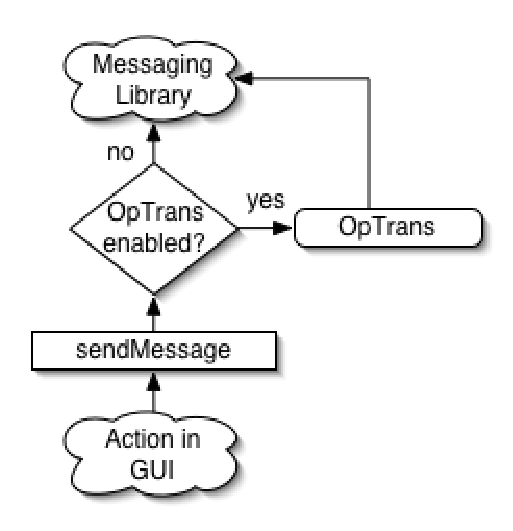
\includegraphics{send.eps}
\caption{Send Filter} \label{send}
\end{center}
\end{figure}

The job of the send filter involves two basic steps.  The first
step is to record the correct \textbf{myMsgs} and \textbf{otherMsgs}
values in the
outgoing message.  The second step is to record the message
in the outgoing list.  These operations are held in case operations
arrive from client sites that were generated before the reception of
our operations.  If this is the case, transformations will be
necessary.  The send filter code is as follows (simplified):

\begin{verbatim}
public void send( MessageEntity msg ) {

  msg.setMyMsgs( this.myMsgs );
  msg.setOtherMsgs( this.otherMsgs );

  this.outgoing.add( msg );
  this.myMsgs++;
}
\end{verbatim}

\textbf{messageReceived} is a public final method in the
\textbf{MessageHandler} class
that acts as an intermediary step between the reception of a message
and its delivery to the \textbf{handleMessage} method.  The
\textbf{handleMessage}
method is not final and is expected to be overridden by subclasses to
provide class specific handling of messages.  Like \textbf{sendMessage},
\textbf{messageReceived} became the obvious place to insert the operational
transformation code that would allow incoming operations to be
processed, and possibly transformed, before being handled locally.
The receive filtering process can be seen in Figure~\ref{receive}.
The \textbf{messageReceived} method is coded as follows:

\begin{verbatim}
public final void messageReceived( MessageEntity msg ) {
  if ( this.opTransEnabled ) {
    OpTrans.getInstance().receive( msg, this ); // receive filter
  }
  else {
    handleMessage( msg );
  }
}
\end{verbatim}

\begin{figure}[!h]
\begin{center}
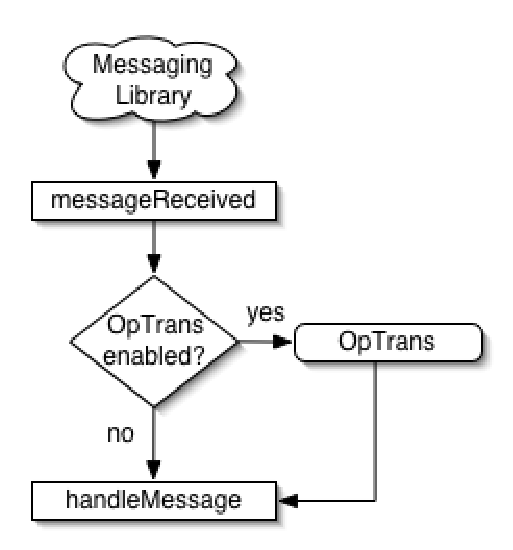
\includegraphics{receive.eps}
\caption{Receive Filter} \label{receive}
\end{center}
\end{figure}

Notice that the receive filter, unlike the send filter, has an extra
parameter other than the actual message.  The second parameter is an
instance of the \textbf{MessageHandler} class.  The reason for the
second parameter is that after transformation the received operation
can be directed back to the correct \textbf{MessageHandler} with a
call to the \textbf{MessageHandler}'s \textbf{handleMessage} method.
If transformation has rendered the operation unnecessary, it is deemed
a no-operation or ``noop,'' and is not forwarded to the
\textbf{handleMessage} call.

The task of the receive filter breaks down into four steps.  The first
step is to discard messages in the outgoing queue that have been
acknowledged by the received message.  If the arriving messages
\textbf{otherMsgs} field has a higher value than a queued messages
\textbf{myMsgs} field
then that message has already been processed by the sending client,
and can therefore be removed.  The next step is for the received
message to be transformed against the messages that remain in the
outgoing queue.  The final two steps involve the forwarding of the
message to the \textbf{handleMessage} method and the increment of the
\textbf{otherMsgs}
field used to track the number of operations completed on behalf of
other clients.  The code is as follows (simplified):

\begin{verbatim}
public void receive( MessageEntity msg, MessageHandler handler ) {
  // discard acknowledged messages in outgoing
  for ( Iterator i = this.outgoing.iterator(); i.hasNext(); ) {
    MessageEntity myMsg = (MessageEntity)i.next();
    if ( myMsg.getMyMsgs() < msg.getOtherMsgs() ) {
      System.out.println( "discarding acknowledged message" );
      i.remove();
    }
  }

  if ( !msg.getAction().equals( "noop" ) ) {
    // transform the new message and the ones in outgoing
    for ( Iterator i = this.outgoing.iterator(); i.hasNext(); ) {
      MessageEntity myMsg = (MessageEntity)i.next();
      OpTrans.xform( msg, myMsg );
    }
  }

  if ( !msg.getAction().equals( "noop" ) ) {
    handler.handleMessage( msg );
  }
  this.otherMsgs++;
}
\end{verbatim}

The active reader may have noticed that the receive operation handles
noop messages and may be wondering why these messages are even sent at
all.  Even though noop messages will cause no changes to the shared
document, they are still useful when they discard messages in the
outgoing queue by acknowledging their receipt.  Also, because a
message that needs to be changed into a noop may be nested several
levels deep, such as within a transaction, it is easier to merely
change it to a noop than it is to remove it from the message
structure.

Several of the above description and code examples have been
simplified to hide the complexity that is introduced by major portions
of the code being shared by both the client and sever instances.  When
operating as a client, only one \textbf{OpTrans} instance must be maintained.
When operating as a server, one \textbf{OpTrans} instance must be kept for each
connected client.  Maintaining separate code bases for client and
server operational transformations would greatly complicate the
process of modifying the operational transformation code.

The solution to this problem was to code the \textbf{OpTrans} class as a
``multiton.''  A multiton is similar to a singleton \cite{gof},
which is a class that allows for only a single instance to be created.
In Java, that instance is typically retrieved with a call to the
\textbf{getInstance} method.  With a multiton, the \textbf{getInstance}
method would
usually receive a parameter, and the parameter would determine which
instance among a set of instances to return to the caller.  From the
design pattern perspective this can be seen as a type of factory
method \cite{gof}.  In the House Party framework, messages
received from the network are disassembled on the client and the
server in the same manner.  When an operation is discovered in a
message that needs to be processed for operational transformations, it
is directed to the correct operational transformation instance as
follows:

\begin{verbatim}
OpTrans.getInstance().receive( msg, this );
\end{verbatim}

On the client side we want this call to retrieve a singleton instance,
while on the server this call needs to retrieve the instance created
for the client that sent the message.  This handled by the server
directing messages through the \textbf{OpTrans} \textbf{serverReceive} call:

\begin{verbatim}
public static void serverReceive( MessageEntity msg, Object client,
    ServerMessagingService msgSvc ) {
  OpTrans.opList.clear();
  OpTrans.activeClient = client;
  msgSvc.messageReceived( msg );
  OpTrans.activeClient = null;
}
\end{verbatim}

As can be seen in the code, the \textbf{OpTrans} \textbf{activeClient}
field is set to
the client that generated the message before the call to
\textbf{messageReceived} with the received message.  As the message travels
down the messaging hierarchy, calls to \textbf{getInstance} can return the
correct \textbf{OpTrans} instance by first checking this field.  If it is null,
then client operation is assumed and the singleton client instance is
returned.  If this field is not null, the instance associated with the
client is returned.  The actual \textbf{getInstance} method is as follows:

\begin{verbatim}
public static OpTrans getInstance() {
  Object key = OpTrans.activeClient != null ? OpTrans.activeClient
      : OpTrans.CLIENT_KEY;
  return OpTrans.getInstance( key );
}
\end{verbatim}

Another case where server and client functionality differs is in the
creation and sending of messages.  When a client sends a message it is
because the user has taken an action on the shared document through
the GUI.  This results in methods being called to do things such as
modify attributes, add entities, and delete entities.  These method
calls make the appropriate changes and then build the message that
will be sent to the server.  The message is then sent with the
\textbf{sendMessage} call.  \textbf{sendMessage} runs the message
through the filter so
that the correct \textbf{myMsgs} and \textbf{otherMsgs} values can
be added to the
message.  The result of the \textbf{sendMessage} call is not necessarily the
message being sent to the server, as an active transaction will cause
the message to merely be added to a transaction message which will
only be sent when the transaction is finished.  The server only
forwards the received message, after possible transformation, on to
the other clients.  This means that the server does not go through the
process of building a message and applying the correct \textbf{myMsgs} and
\textbf{otherMsgs} values for each client.  This must be done, however, before
the message can be forwarded to the connected clients.

The solution to this problem was to keep a linked list of the
operations subject to operational transformation as they are parsed
out of the received message.  The code that performs this task can be
seen in the \textbf{OpTrans} receive method:

\begin{verbatim}
if ( OpTrans.activeClient != null ) {
  OpTrans.opList.add( contentMsg );
}
\end{verbatim}

Because it is unnecessary to do this on the client, the presence of an
active client can be used to determine if we are running as a server
or a client.

With the \textbf{opList} linked list storing references to the
operations subject to operational transformations, we can then set the
\textbf{myMsgs} and \textbf{otherMsgs} values to the correct values
for each client before forwarding the message on to that client.  This
is done by preparing the message in the \textbf{serverSend} call
before the actual sending of the message with the messaging libraries
\textbf{writeMessage} call.  The \textbf{serverSend} call works by
first retrieving the correct \textbf{OpTrans} instance for the client
that it is about to send a message to.  After that, a loop iterates
through the operations referenced in the linked list \textbf{opList},
setting the \textbf{myMsgs} and \textbf{otherMsgs} values properly for
that client.  The \textbf{serverSend} code is as follows:

\begin{verbatim}
public static void serverSend( Object client ) {
  OpTrans opTrans = OpTrans.getInstance( client );

  for ( Iterator i = OpTrans.opList.iterator(); i.hasNext(); ) {
    MessageEntity msg = (MessageEntity)i.next();
    msg.setMyMsgs( opTrans.myMsgs );
    msg.setOtherMsgs( opTrans.otherMsgs );

    opTrans.outgoing.add( msg.clone() );
    opTrans.myMsgs++;
  }
}
\end{verbatim}

The techniques described above allow the majority of the operational
transformation code in the Loose Dog system to be shared by client and
server instances.  This is a great benefit to the future
maintainability of the Loose Dog code base.

The last step in completing the operational transformation system was
to code the actual transform functions.  These are the functions that
must be executed when the ordering of operations cannot be
determined.  For a system with \emph{m} operations, an
\emph{m}x\emph{m} matrix, referred to as the transformation matrix,
must be built.  Each component of the matrix is a transformation
function where the row header indicates the type of client operation
and the column header indicates the type of server operation.  A
representation of the matrix can be seen in Figure~\ref{matrix}.

\begin{figure}[!h]
\begin{center}
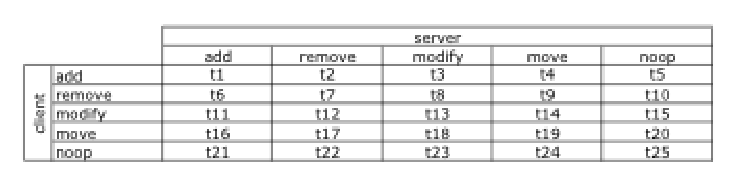
\includegraphics{matrix.eps}
\caption{Transformation Matrix} \label{matrix}
\end{center}
\end{figure}

Many of these functions result in no transformation to
the given operations (all of the operations involving noop).
As an example, consider the case where one
client moves an entity while another changes an attribute on an
entity.  In this case neither operation interferes with the other and
therefore no transformation is needed.  As a counter example, consider
the case where two clients move an entity.  In this case the transform
function must check if it is the same entity, and if it is, one of the
move operations must be declared the winner.  In the cases where the
operation is considered atomic I have gone with the client whose
operation reached the server first to be the winner.

\section{Conclusion}

I am very pleased with the implementation of the operational
transformation component of the Loose Dog system.  The system was
integrated into the exiting House Party framework with a minimal
amount of modifications to the existing code.  Part of this is due to
the effective modularization of the operational transformation code,
however, much of it is also due to the architecture of the House Party
framework primarily engineered by Nathan Dwyer.  Loose Dog operational
transformations has been delivered with a very understandable code
base which is going to be a big benefit to anyone
who works with House Party and Loose Dog in the future.

With that being said, much work is left to be done with the House
Party framework and Loose Dog system.  At this point in time the
system has undergone very little stress testing to identify and hammer
out any lingering bugs.  In particular, the Loose Dog system needs to
be checked for possible race conditions that may exist when the
production of an outgoing message with operational transformations is
interrupted by an incoming message.

Loose Dog now provides House Party with the communications and
synchronization abilities needed to build an effective distributed
collaborative framework.  It will be very interesting to see where
House Party pops up and Loose Dog wanders off to in the future.

\newpage

\begin{thebibliography}{99}
\bibitem{grove} C. A. Ellis, S. J. Gibbs: \emph{Concurrency Control in
  Groupware Systems}, In \emph{Proc. of ACM SIGMOD Conference on Management
  of Data}, pp. 399-407, 1989.
\bibitem{reduce} C. Sun, X. Jia, Y. Zhang, and Y. Yang: \emph{A
  generic operation transformation scheme for consistency maintenance
  in real-time cooperative editing systems}, In \emph{Proc. of ACM
  Conference on Supporting Group Work}, pp. 425-434, Nov. 1997.
\bibitem{jupiter} D. Nichols, P. Curtis, M. Dixon, and J. Lamping:
  \emph{High-latency, low-bandwidth windowing in the Jupiter
  collaboration System}, In \emph{Proc. of ACM Symposium on User Interface
  Software and Technologies}, pp. 111-120, Nov. 1995.
\bibitem{adopted} M. Ressel, D. Nitsche-Ruhland, and R. Gunzenbauser:
  \emph{An integrating, transformation-oriented approach to
  concurrency control and undo in group editors}, In \emph{Proc. of
  ACM Conference on Computer Supported Cooperative Work}, pp. 288-297,
  Nov. 1996.
\bibitem{subetha} D. Wagner, M. Ott, M. Pittenauer, U. Bauer, P. Broz,
http://www.codingmonkeys.de/subethaedit/, May 2004.
\bibitem{livemeeting} Microsoft, http://main.placeware.com/
\bibitem{gof} E. Gamma, R. Helm, R. Johnson, J. Vlissides,
  \emph{Design Patterns - Elements of Reusable Object-Oriented
  Software}, Addison-Wesley, Reading, MA, 1995.

\end{thebibliography}

\end{document}
